\section{Problem 4}

\subsection{Matlab Code Method}
The Matlab code for this homework problem was broken up into multiple functions and scripts so that they could easily be used in future problems.
There were 3 Matlab scripts used for this analysis: homework4\_q4.m, pattern\_generator.m, uniformarraypattern.m, and directivity.m .
\subsubsection{homework4\_q4.m}
homework4\_q4.m is the main script for this problem. 
It uses the other helper scripts to produce the final graphs and verification of the results. 
The script starts by defining the element spacings $d$, total number of elements $N$, and phase shift $\beta = beta$ to be plotted. It also defines the angle step sizes for pattern simulation ($dtheta$ and $dphi$). 

Then for each of the distances and phase shifts, it calls the pattern\_generator script with the uniformarraypattern function handle. 
The produced patterns are then passed to the directivity script which numerically integrates to calculate the directivity.
For specific phase shifts, the numerically integrated results are compared to the expected value produced by the directivity formula.
\subsubsection{pattern\_generator.m}
The pattern generator script takes in angle step sizes, a function handle, and varargin (any other necessary parameters for the function handle). The function passed through its function handle (this is achieved using @function\_name in the script calling pattern\_generator) is the desired pattern function to be evaluated..
The passed function is evaluated over all of $\theta$ and $\phi$ and an array of the pattern and angles is returned to the calling function.  
\subsubsection{directivity.m}
The directivity function takes in $\theta$, $\phi$ and a corresponding pattern and then numerically integrates to calculate the directivity of that pattern.
\subsubsection{unifrormarraypattern.m}
This script returns the array factor for a given uniform array described by the number of elements, element spacing, phase shift, $\theta$, and $\phi$.

\subsection{Results: Directivity vs Phase Shift}
The following graphs display the directivity vs phase shift for a 10 element uniform array at element spacings of [0.5 0.4 0.1] $\lambda$ .
They were produced using the numerical integration Matlab script I wrote mentioned above. For these 3 spacings, the directivity for 1000 different phase shifts was calculated.

The one oddity I saw in my results was that for d = 0.5 $\lambda$ there initially appeared to be a lot of variability from the expected result of a constant 10. Upon a closer look, the max difference was less than 0.015 and the variability could be explained as just a small limitation caused by using a limited number of points for the numerical integration.

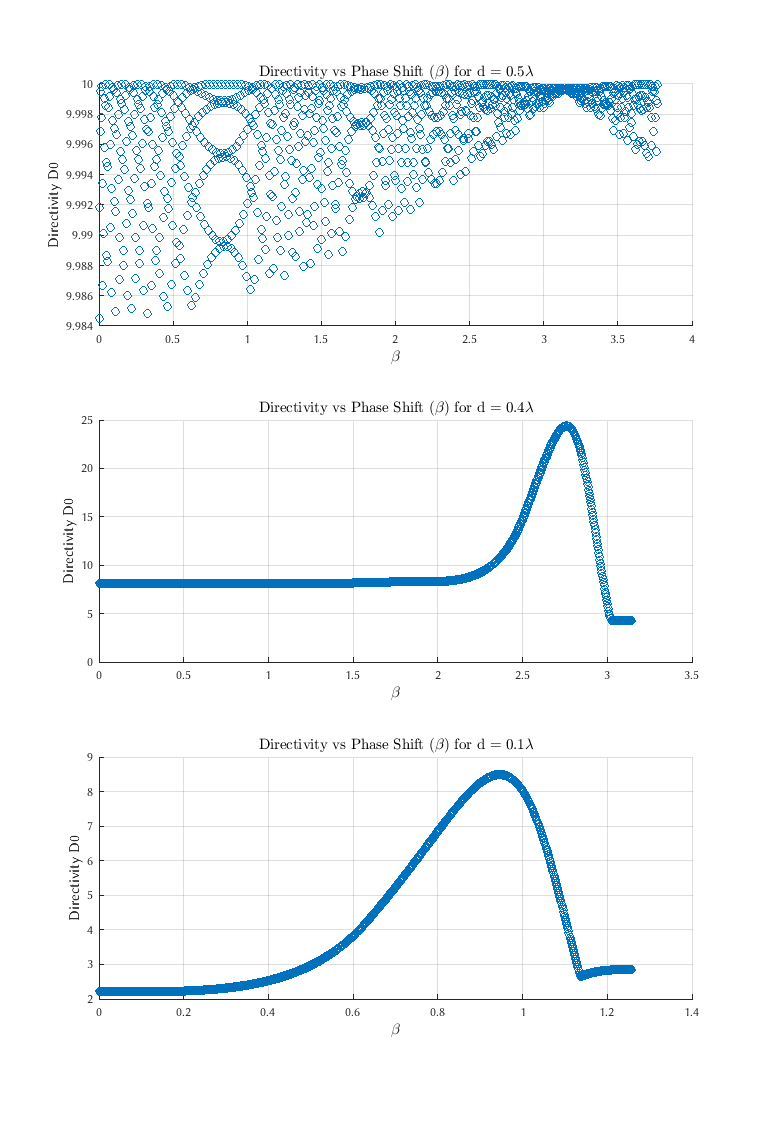
\includegraphics[scale=.7]{homework4_3graphs.png}

\subsection{Verification}
To verify my results, I programmed a directivity formula based off of solid angles. $D_0 = \frac{4*\pi}{\Omega}$.

\begin{equation}
	D = \frac{(norm)}{\frac{1}{N} + \frac{1}{N^2}* \sum_{m=1}^{N-1}\frac{N-m}{mkd}*sin(mkd)*cos(m\beta)}
\end{equation}

For	$ \delta = [\beta - k*d , \beta +k*d] $
\begin{equation}
	norm = max(\Bigg|\frac{sin(N\delta/2)}{N*sin( \delta/2)}\Bigg|^2) 
\end{equation}


I compared my numerical integration results to those produced by the formula. They align very well with only minor errors. Thus, I feel confident that my numerical integration is working properly.

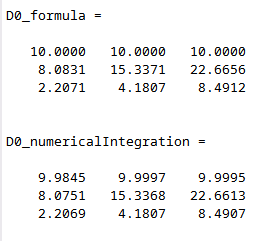
\includegraphics[scale=1]{hw4_verification.png}

